\PassOptionsToPackage{unicode, colorlinks=true, linkcolor=black, urlcolor=black}{hyperref}
\documentclass[t, table]{beamer}

%% load the theme with the correct option for your institute
%% currently supported are tudo and ethz
\usetheme{fact}

\usepackage[
  orientation=portrait,
  size=a0,
  scale=1.0,  % scale fonts with this factor
]{beamerposter}

\usepackage{fontspec}
\usepackage{polyglossia}
\setmainlanguage[variant=american]{english}

% microtypographic adjusments (protrusion, kerning etc.)
\usepackage{microtype}

% automatic enquoting depending on the language with \enquote{Bla}
\usepackage{csquotes}

% for the qrcode
\usepackage{qrcode}

% math setup
\usepackage{mathtools}
\usepackage{unicode-math}
\setmathfont[Scale=MatchLowercase]{TeX Gyre Pagella Math}

\usepackage{xfrac}
\usepackage[
  detect-weight=true,
  binary-units=true,
  per-mode=fraction,
  fraction-function=\sfrac
 ]
 {siunitx}
% some stupid sample text to fill the boxes
\usepackage{blindtext}

% offers the \begin{multicols}{NCOLS} environment
\usepackage{multicol}

% for including all types of graphics
\usepackage{graphicx}

\usepackage{tabularx}

% bibliography settings
\usepackage[
  backend=biber,
  style=numeric,
  url=false,
  sorting=none,
  firstinits=true,
]{biblatex}
\DeclareFieldFormat*{title}{\textit{#1}}


\newcommand{\stf}{\texttt{streams-framework} }
% a little complicated, but this creates an inline list.
\renewcommand*{\bibfont}{\footnotesize}
\addbibresource{references.bib}
\defbibenvironment{bibliography}
  {\noindent}
  {\unspace}
  {}
\renewbibmacro*{begentry}{%
  \usebeamercolor{bibliography item}%
  \color{bibliography item.fg}%
  \printtext[labelnumberwidth]{%
    \printfield{prefixnumber}%
    \printfield{labelnumber}%
  }%
  \setunit{\addnbspace}%
}
\renewcommand*{\finentrypunct}{\addperiod\space}

% just a helpful definition to get columns with a third of the textwidth
\newlength{\thirdtextwidth}
\setlength\thirdtextwidth{0.333333\textwidth}


\title{Distributed Real-Time Data Stream Analysis for CTA}
\author{Kai Brügge and Alexey Egorov}
\newfontfamily{\firathin}{fira sans thin}
\usetikzlibrary{calc}
\usetikzlibrary{shadows.blur}

\begin{document}%

\begin{multicols}{2}
    \begin{block}[]{CTA - The Cherenkov Telescope Array}%
      \begin{multicols}{2}
        \begin{figure}
          \includegraphics[width=\linewidth]{images/cta.png}\\
          % \caption{The FACT Telescope during a calibration procedure \cite{fact-performance}}
        \end{figure}
        \columnbreak
        Once completed, the  Cherenkov Telescope Array (CTA)  will be able to map the gamma-ray sky
        in a wide energy range from several tens of GeV to some hundreds of TeV and will be more sensitive
        than previous experiments by an order of magnitude.

        CTA will consist of approximately 100 telescopes of different sizes and designs.
        Telescope data will be streamed via network from the telescopes to a central computing facility
        on-site.
      \end{multicols}
    \end{block}%

    \begin{block}[]{Monitoring the Gamma-Ray Sky}%
      \begin{multicols}{2}
        \begin{figure}
          \includegraphics[width=\linewidth]{figures/fermi.pdf}\\
          % \caption{Toller Plot.\cite{fact-performance}}
        \end{figure}
        \columnbreak
        One of CTA's main goals is monitoring the sky for transient events. These include Gamma-Ray Burst (GRBs) events and
        Active Galactic Nuclei (AGNs).
        To gain more understanding about the physics behind GRBs and AGN it is vital to perform multi-wavelengths observations.
        In case a GRB is detected,  CTA can alert other experiments to trigger observations in other wavelengths bands.
        The figure to the left shows all GRB events collected during 6 years of operation of the Fermi satellite\cite{fermi}.
      \end{multicols}
    \end{block}%
    %
    % \begin{block}[equal height group=B]{\stf}%
    %   \begin{multicols}{2}
    %     \begin{figure}
    %       \includegraphics[width=\linewidth]{images/cta.png}\\
    %       % \caption{The FACT Telescope during a calibration procedure \cite{fact-performance}}
    %     \end{figure}
    %     \columnbreak
    %       The \stf is a data streaming environment written in Java.
    %       The purpose of the streams-framework is to provide an abstract way to model the data flow of an application.
    %       It comes with a number of fundamental building blocks to define a data flow graph using an Extensible Markup Language (XML) based description.
    %       Programms written within the \stf can be executed on distributed computing engines such as Apache Storm, Flink and Spark.
    %   \end{multicols}
    % \end{block}%


    \begin{block}[]{Classification and Regression}%
      \begin{multicols}{2}
          \begin{figure}
            \includegraphics[width=0.9\linewidth]{figures/stream.pdf}\\
          \end{figure}
        \columnbreak
        Supervised machine learning is used to separate signal from background and to estimate
        the energy of a recorded event. Features for classification/regression are calculated from raw input
        images.
        Simulated, labeled, data is used to train the models using the Python machine learning library scikit-learn\cite{sklearn}.
        The trained scikit-learn models are converted into the PMML\cite{pmml} format using the sklearn2pmml\cite{sklearn2pmml} library.
        This way the stored model can be shared
        between programming languages and applied to the data stream from the telescopes.
      \end{multicols}
    \end{block}%

    \begin{block}[]{Framework Comparisons}%
      \begin{multicols}{2}
        \begin{figure}
          \includegraphics[width=\linewidth]{figures/eventrate_vs_framework.pdf}\\
          % \caption{Toller Plot.\cite{fact-performance}}
        \end{figure}
        \columnbreak
        Tuning the Apache Spark framework for fast streaming application is more complicated due to its micro-batch architecture.
        Hence, we concentrated on Apache Storm\cite{storm} and Apache Flink\cite{flink}. We compare the runtime of Storm, Flink and the streams-framework\cite{streams} in
        a local setup on a single core to measure the impact of the overhead these frameworks produce.
        The results can be seen on the image on the left.
        There is no clear preference between Storm and Flink when it comes to runtime overhead. We chose to continue our experiments on
        Apache Flink due to easier setup, better visualization tools and a more comfortable abstraction compared to the rather low-level
        API of Apache Storm.
      \end{multicols}
    \end{block}%

    \begin{block}[]{Runtime Measurements}%
      \begin{multicols}{2}
        \begin{figure}
          \includegraphics[width=\linewidth]{figures/runtime.pdf}\\
          % \caption{Toller Plot.\cite{fact-performance}}
        \end{figure}
        \columnbreak
          The figure on the left shows the number of events per second versus the number of used CPU cores.
          This test was executed on a machine with 24 physical CPU cores and 128 Gigabytes of RAM.
          The datarate goes up to approximately \num{14000} events per second. The expected eventrate of CTA is between
          \num{10000} and \num{20000} events per second depending on deployment\cite{trigger}.
          This shows that it will be possible to completely analyse CTA data with only a few of computers.
          Frameworks like Apache Flink allow for simple and maintable workload distribution with fault tolerance and high availability mechanisms to recover from hardware, network or further failures.
%          Furthermore, fault tolerance and high availability features  and  make distributing the workload over many computers simple and maintanable.
      \end{multicols}
    \end{block}%


% ------------------Next columns -----------------
% ------------------------------------------------
    \columnbreak

        \begin{center}

        \begin{streamblock}[equal height group=C, width=0.8\linewidth]{0mm}{-5mm}{}%
          \begin{multicols}{2}
            \begin{figure}
              \includegraphics[width=\linewidth]{figures/trigger.pdf}
            \end{figure}
            \columnbreak
            Images from all telescopes in the array get collected into a central trigger where images belonging together are merged into so called events.
            This way each image gets a unique event id.
            CTA emits up to \num{15 000} events per second\cite{trigger}.
          \end{multicols}
        \end{streamblock}%

        \begin{streamblock}[colframe=white!60!black, height=2.1cm, width=0.8\linewidth]{-5mm}{0mm}{}%
          \begin{center}
            Distribute images throughout cluster.
          \end{center}
        \end{streamblock}%

        \begin{streamblock}[equal height group=C, width=0.8\linewidth]{0mm}{-5mm}{}%
          \begin{multicols}{2}
            % \rowcolors{2}{gray!25}{white}
            % {\color{maincolor}
            % \begin{tabularx}{\linewidth}{cccc}
            %   \rowcolor{gray!50}
            %     \textbf{Length} & \textbf{Width} & \textbf{Size} & \textbf{EventID} \\
            %     30 & 15   & 100   & 1\\
            %     40 & 10  & 200  & 1\\
            %     29 & 25  & 75  & 1\\
            %     40 & 30  & 500 & 3\\
            %     5 & 2  & 12 & 5\\
            %     20 & 13  & 84 & 3
            % \end{tabularx}
            % }
            \begin{figure}
              \includegraphics[width=\linewidth]{figures/image.pdf}
            \end{figure}

            \columnbreak
            Each image in the event has to be converted into feature representation before classification and regression.
            Due to the parallel nature of the processing, the processed images do not necessarily retain their order.
            At this stage per-telescope operations can be applied.

          \end{multicols}
        \end{streamblock}%

        \begin{streamblock}[equal height group=C, width=0.8\linewidth]{-5mm}{-5mm}{}%
          \begin{multicols}{2}
            \begin{figure}
              \includegraphics[width=\linewidth]{figures/auc_type.pdf}
            \end{figure}
            \columnbreak

            At this stage the pre-trained machine learning models can be applied since they
            have been trained on single telescope data. The plot on the left shows the performance
            of background suppression for a single telescope.

          \end{multicols}
        \end{streamblock}%


        \begin{streamblock}[height=2.1cm, colframe=white!60!black,, width=0.8\linewidth]{-5mm}{0}{}%
          \begin{center}
            Collect results from an event using a fixed time window.
          \end{center}
        \end{streamblock}%

        \begin{streamblock}[equal height group=C, width=0.8\linewidth]{0mm}{-5mm}{}%
          \begin{multicols}{2}
            \begin{figure}
              \includegraphics[width=\linewidth]{figures/total_auc.pdf}
            \end{figure}
            \columnbreak
            Predictions for a single telescope are averaged to get a better predictor.
            The plot on the left shows the area under the reciever operating characteristic.
            Compared to the single telescope prediction it improves background rejection significantly.
          \end{multicols}
        \end{streamblock}%

        \begin{streamblock}[equal height group=C, width=0.8\linewidth]{-5mm}{-5mm}{}%
          \begin{multicols}{2}
            \begin{figure}
              \includegraphics[width=\linewidth]{figures/resolution.pdf}
            \end{figure}
            \columnbreak
            The direction of the air shower is reconstructed from the features calculated in the previous step.
            The plot on the left shows the angular resolution of the reconstruction for different energy bands.
            As expected the error on the reconstruction decreases for brighter events.
          \end{multicols}
        \end{streamblock}%

        \begin{streamblock}[equal height group=C, width=0.8\linewidth]{-5mm}{0}{}%
          \begin{multicols}{2}
            \begin{figure}
              \includegraphics[width=\linewidth]{figures/skymap.pdf}
            \end{figure}
            \columnbreak
            At this point the reconstructed gamma-ray events can be used for analysis.
            The reconstructed events can be collected into a histogram of sky coordinates.
            The image on the left shows a skymap for a simulated gamma-ray source.
          \end{multicols}
        \end{streamblock}%
        \vspace{2cm}
        \begin{multicols}{2}
            \begin{figure}
              
\includegraphics[width=\linewidth]{logos/github.png}
            \end{figure}
            \columnbreak
                \vspace*{2cm}
                \begin{tabular}{l}
                https://github.com/mackaiver/jayct \\
                https://github.com/mackaiver/streams-cta
                \end{tabular}




          \end{multicols}


      \end{center}

\end{multicols}


\vfill
\begin{columns}[t, onlytextwidth]%
  \begin{column}{0.50\textwidth}%
    \begin{block}[equal height group=bottom]{\normalsize References}
      \footnotesize%
      \printbibliography%
    \end{block}
  \end{column}%
  \begin{column}{0.20\textwidth}%
    \begin{block}[equal height group=bottom]{\normalsize Acknowledgment}
        \footnotesize
        Part of this work is supported by Deutsche Forschungsgemeinschaft (DFG) within the Collaborative Research Center SFB 876
"Providing Information by Resource-Constrained Analysis", project C3. 

    \end{block}
  \end{column}%
  \begin{column}{0.30\textwidth}%
    \begin{block}[equal height group=bottom]{\normalsize Contact}
      \begin{columns}[T]
        \begin{column}{0.2\textwidth}
              \begin{figure}
                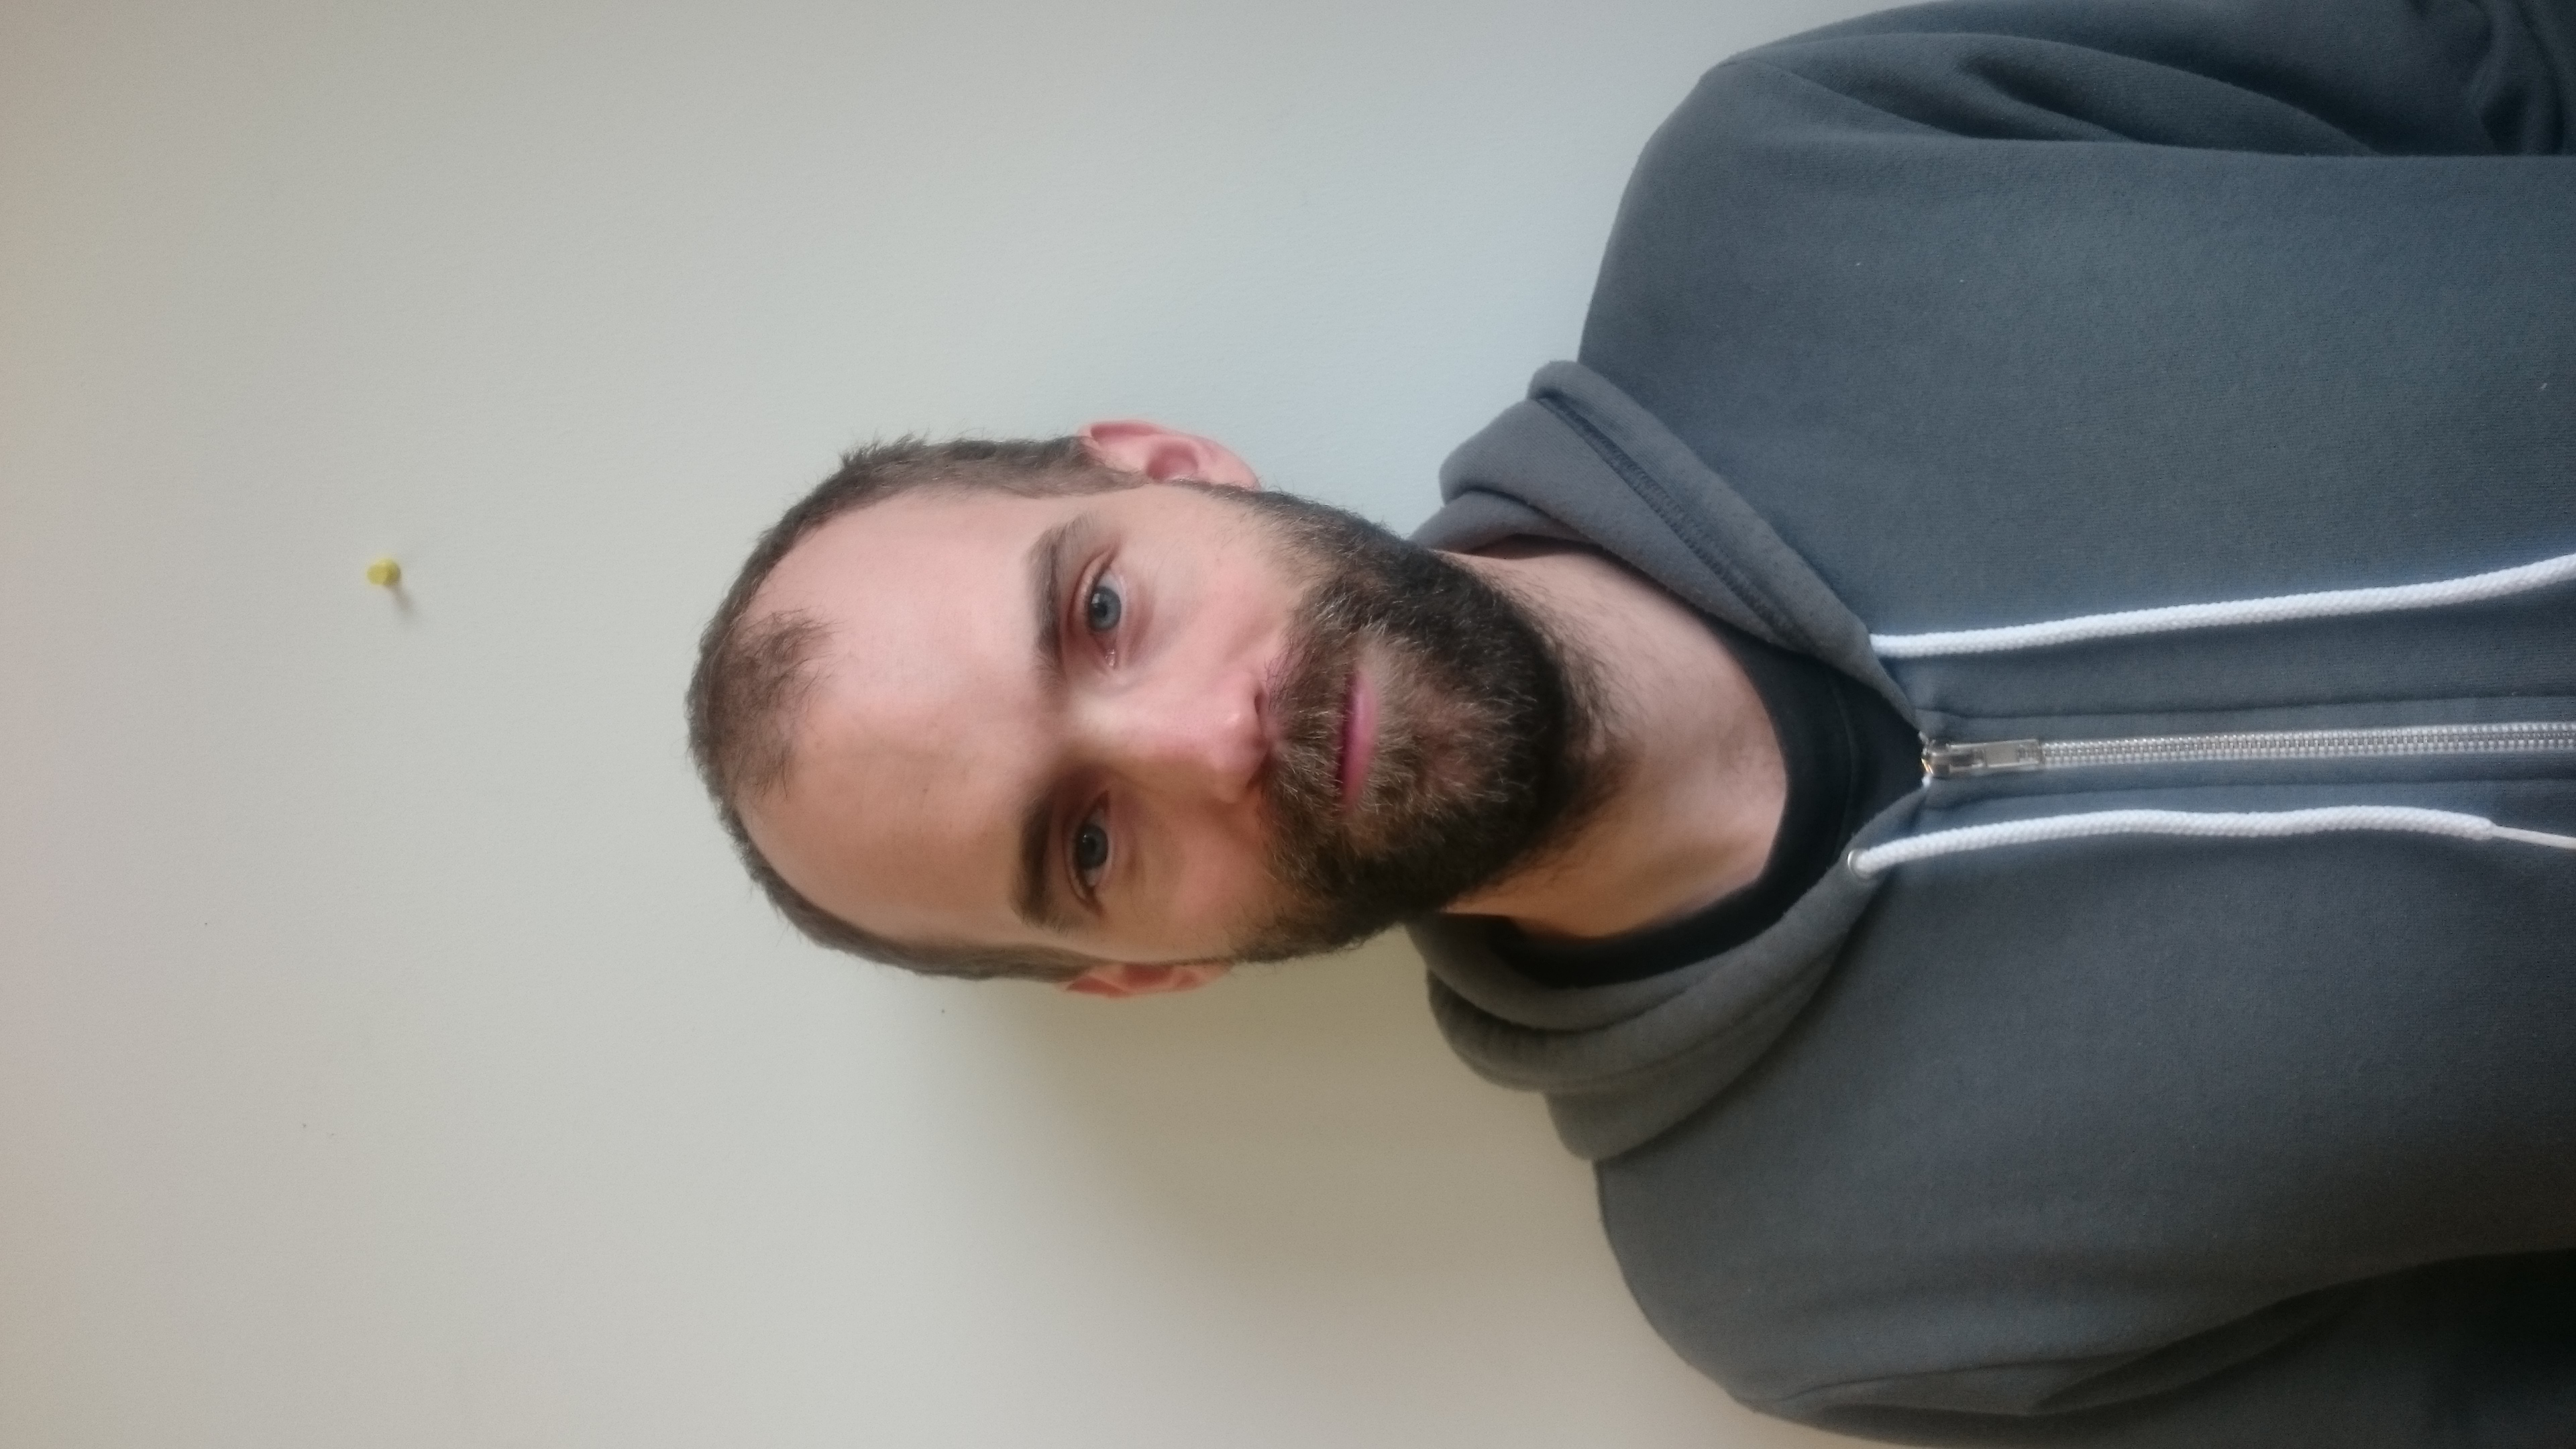
\includegraphics[width=1.2\linewidth, angle=-90]{images/kai.jpg}
              \end{figure}
        \end{column}
        \begin{column}{0.3\textwidth}
            \footnotesize
                     \vspace*{0.5cm}
                Kai Brügge, \\
                Astroparticle Physics, \\
                TU Dortmund \\
                \texttt{kai.bruegge@udo.edu}
        \end{column}
        \begin{column}{0.2\textwidth}
              \begin{figure}
                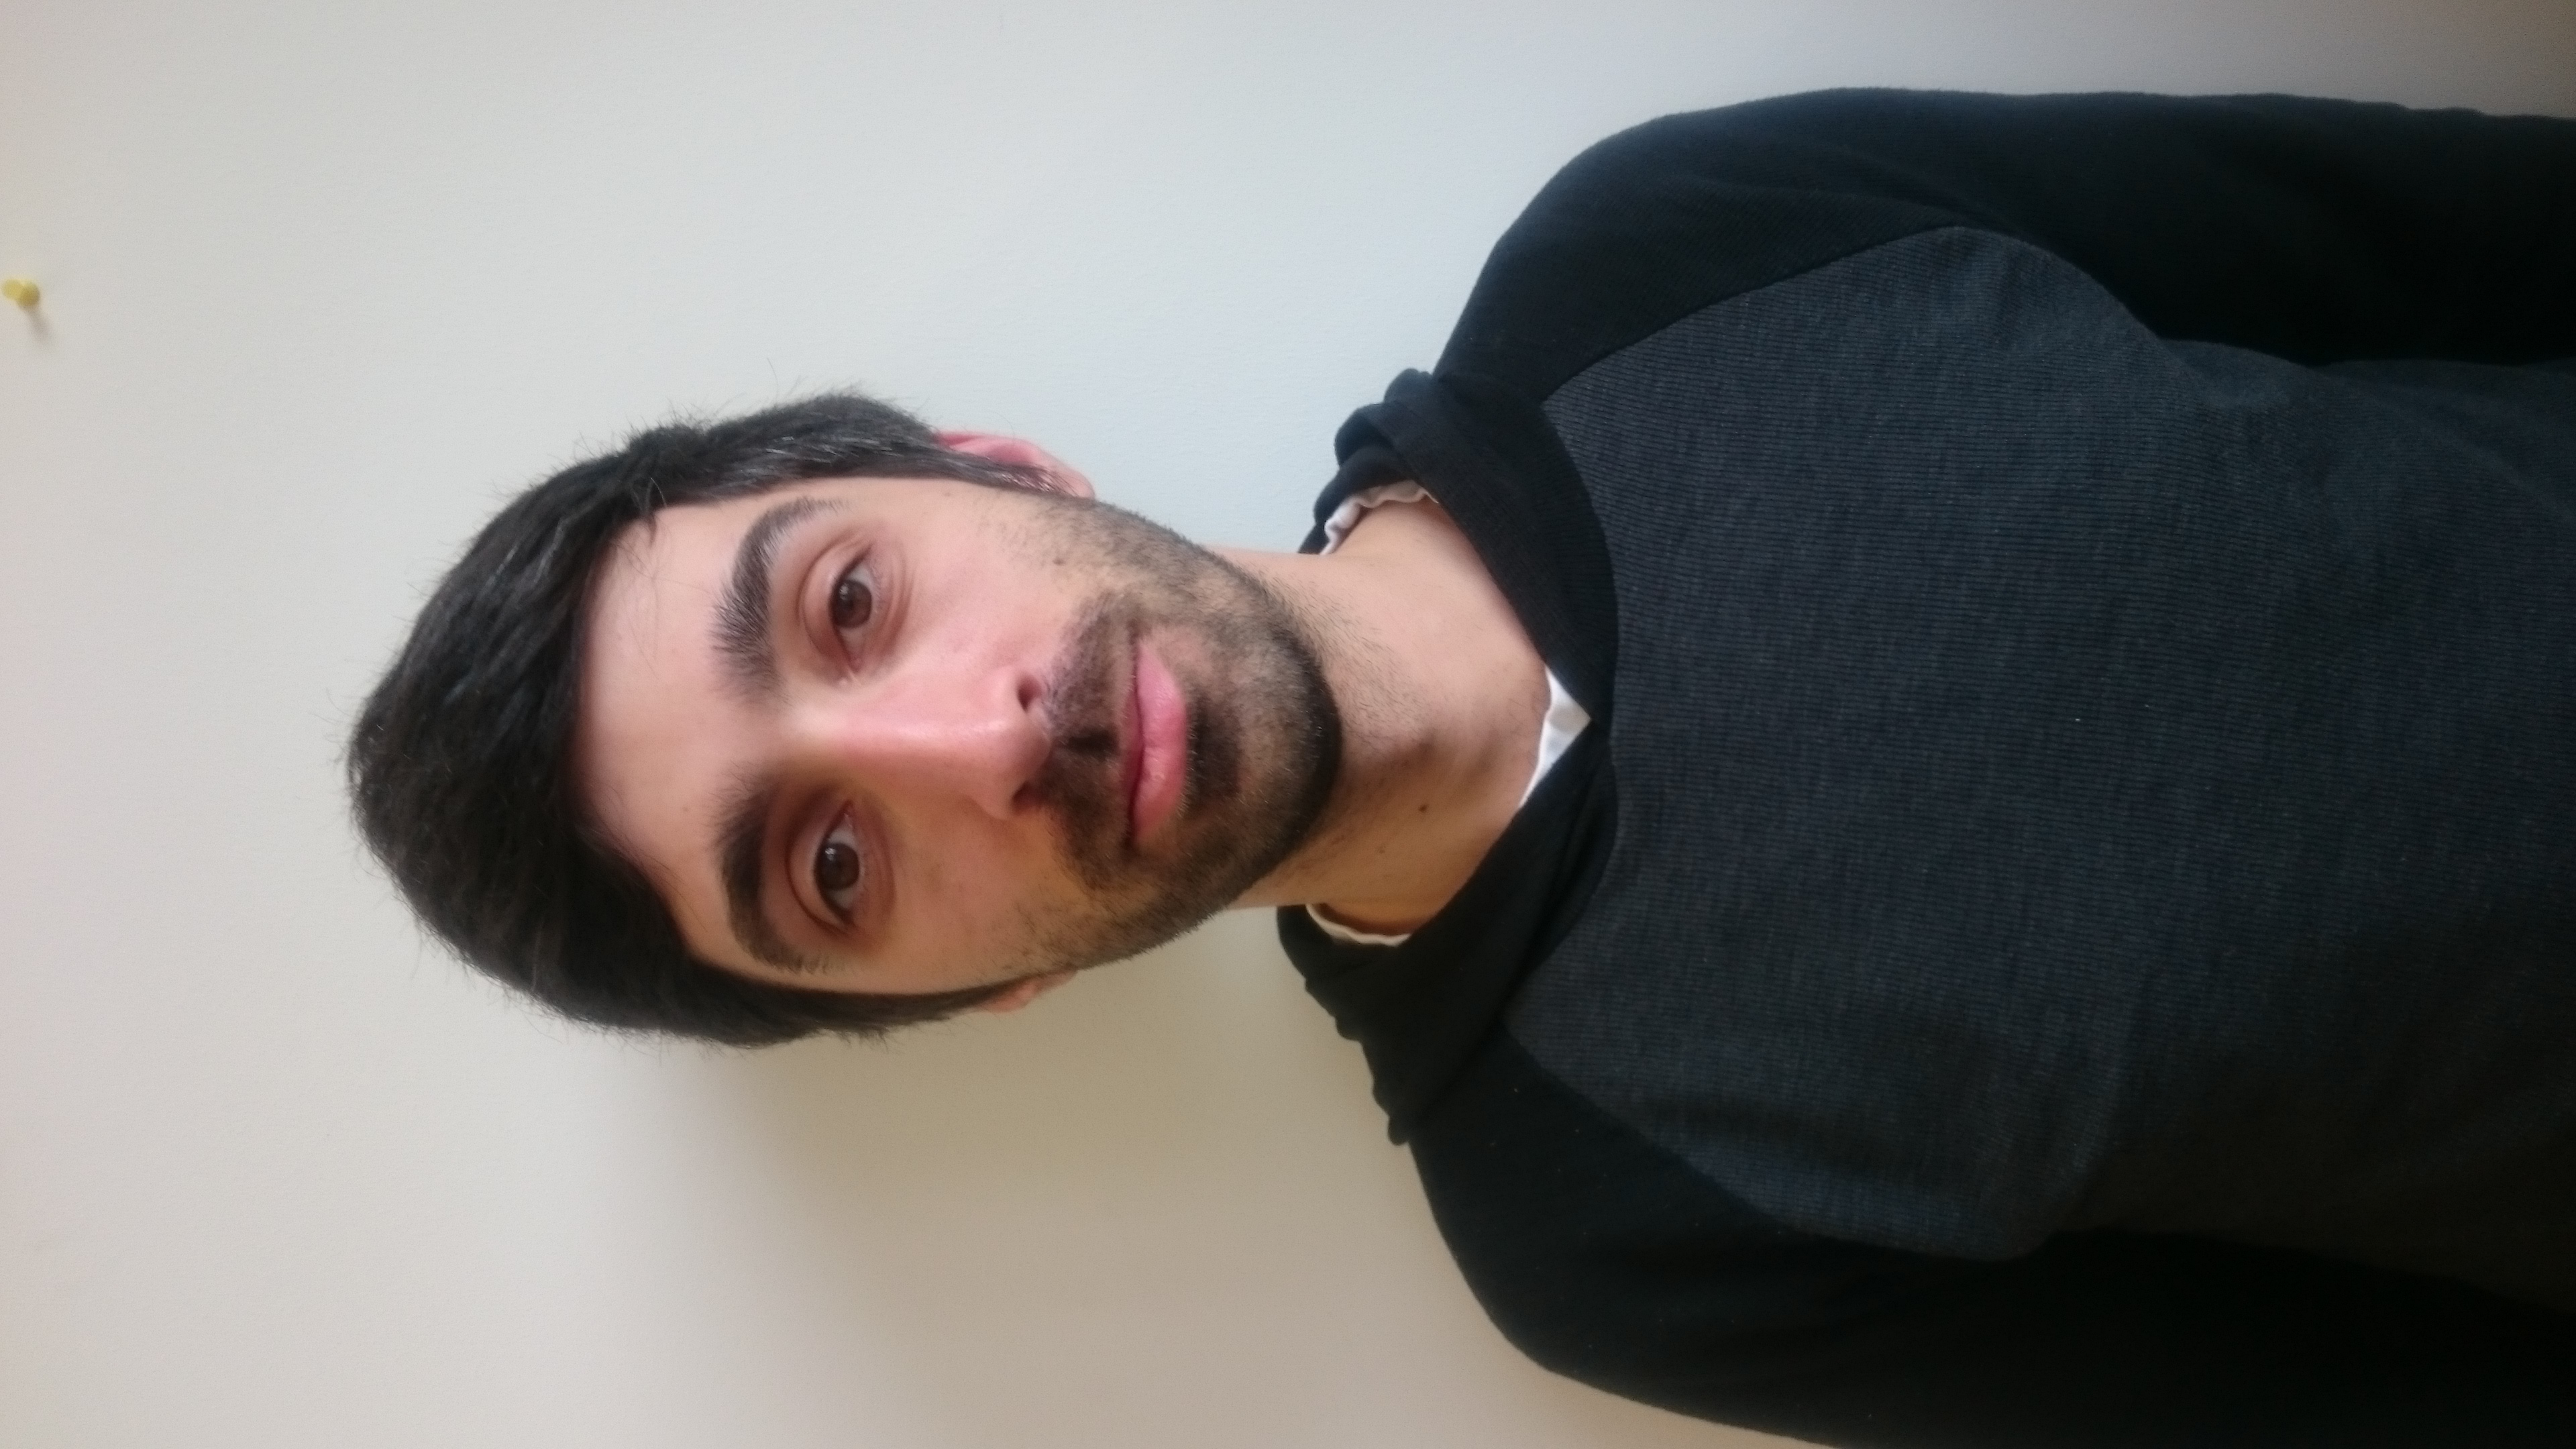
\includegraphics[width=1.2\linewidth, angle=-90]{images/alexey.jpg}
              \end{figure}
        \end{column}
        \begin{column}{0.3\textwidth}
              \footnotesize
                  \vspace*{0.5cm}
                  Alexey Egorov, \\
                  AI Group, \\
                  TU Dortmund \\
                  \texttt{alexey.egorov@udo.edu}
        \end{column}
      \end{columns}

      % \begin{multicols}{4}
      %     \begin{figure}
      %       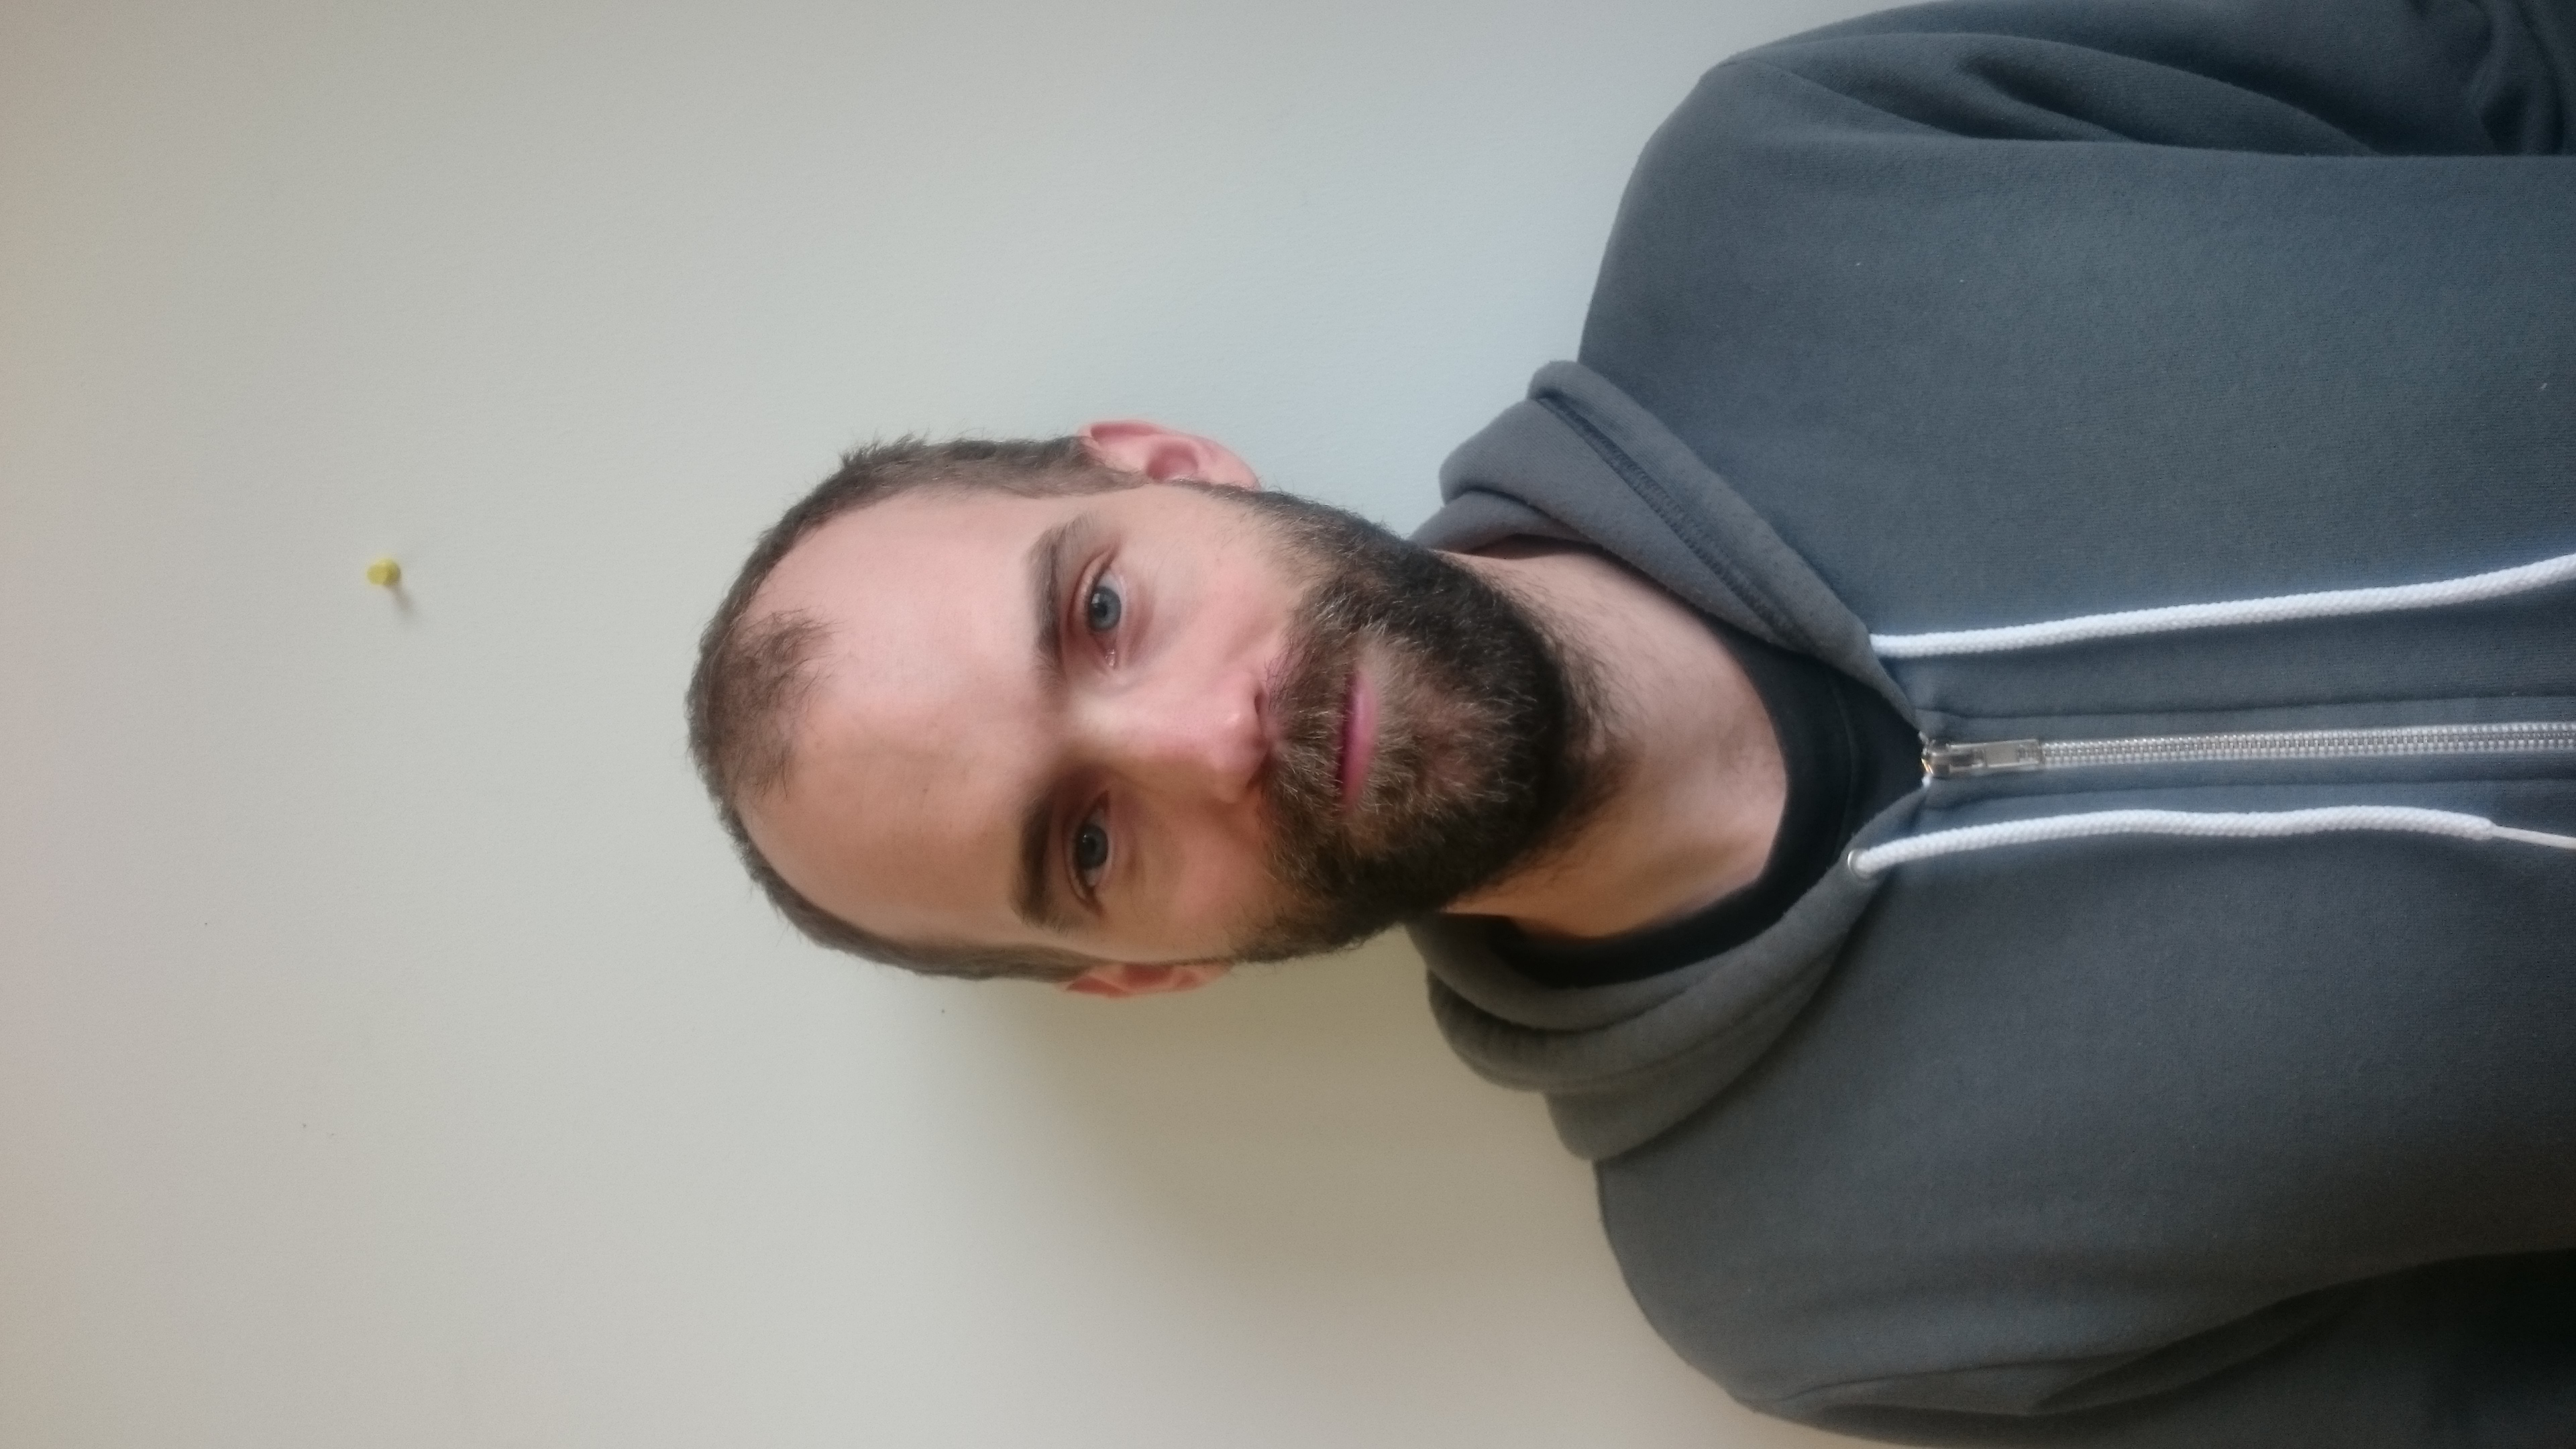
\includegraphics[width=0.7\linewidth, angle=-90]{images/kai.jpg}
      %     \end{figure}
      %     \columnbreak
      %         \footnotesize
      %             Kai Brügge, \\
      %             Astroparticle Physics, \\
      %             TU Dortmund \\
      %             \texttt{kai.bruegge@udo.edu}
      %     \columnbreak
      %       \begin{figure}
      %         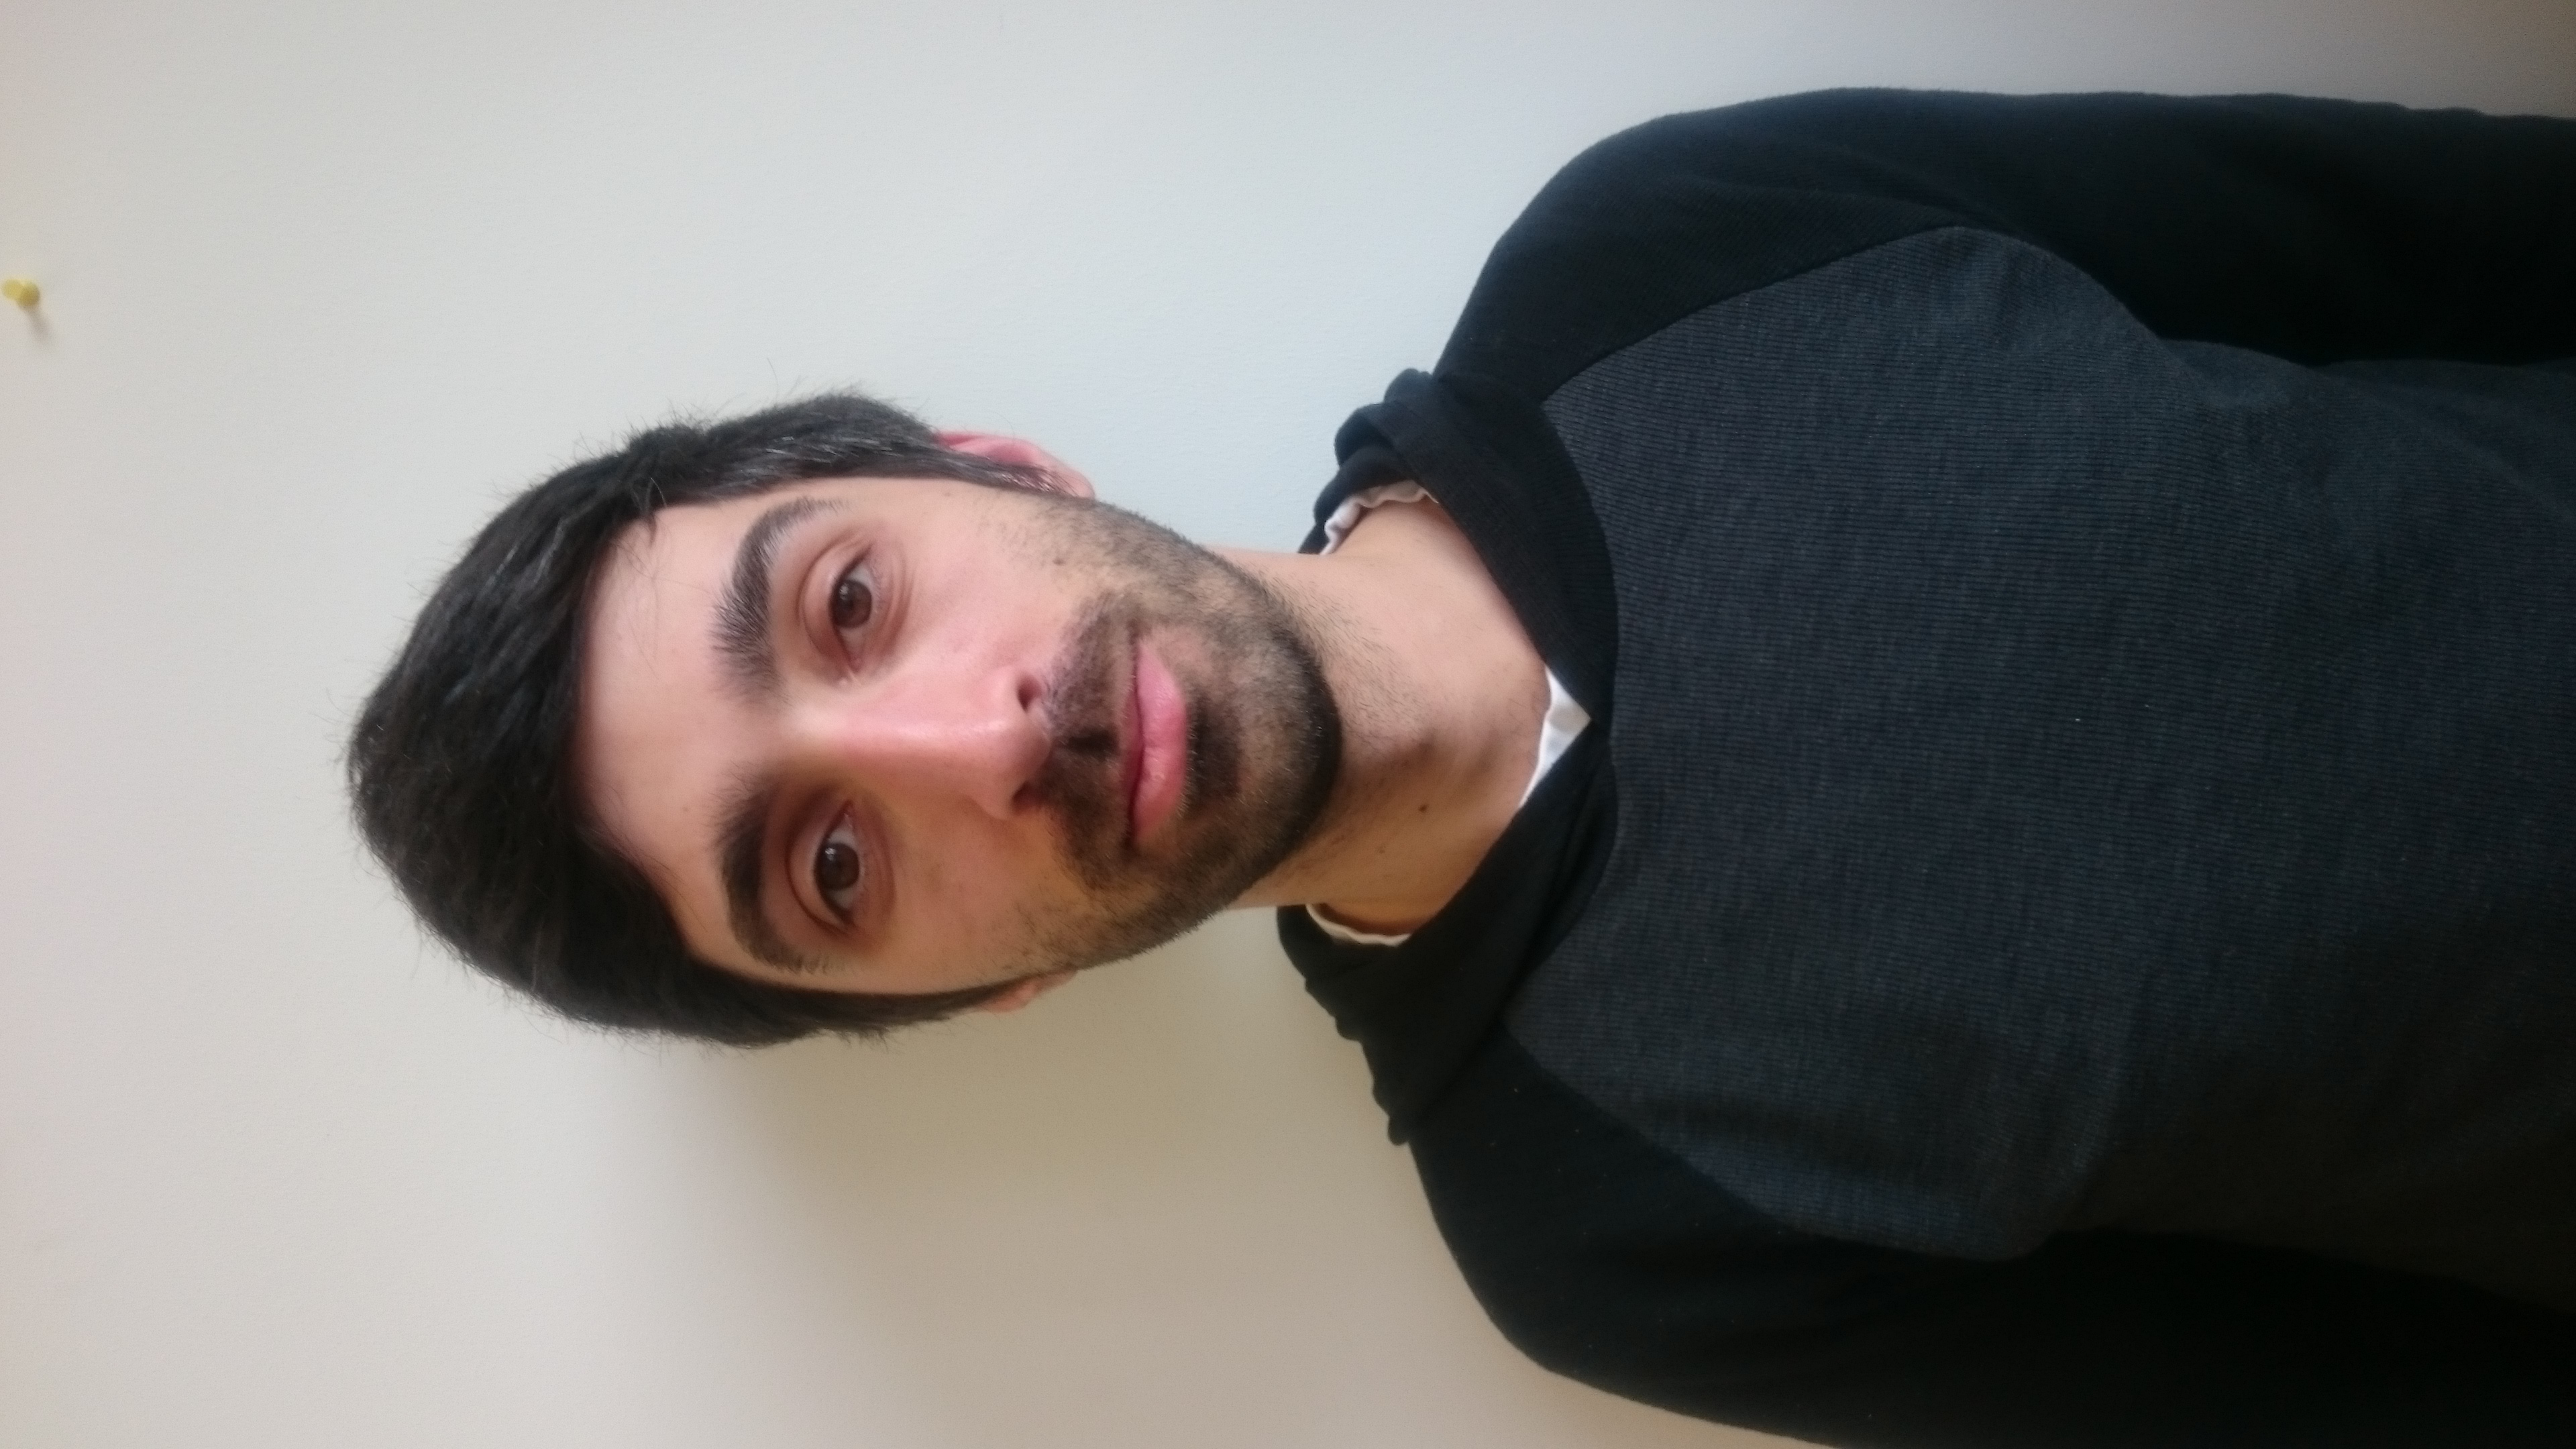
\includegraphics[width=0.7\linewidth, angle=-90]{images/alexey.jpg}
      %       \end{figure}
      %       \columnbreak
      %           \footnotesize
      %               Alexey Egorov, \\
      %               AI Group, \\
      %               TU Dortmund \\
      %               \texttt{alexey.egorov@udo.edu}
      %   \end{multicols}
      % \begin{columns}%
      %   \begin{column}{0.18\linewidth}
      %     \tikz[]{
      %       \node[anchor=north]{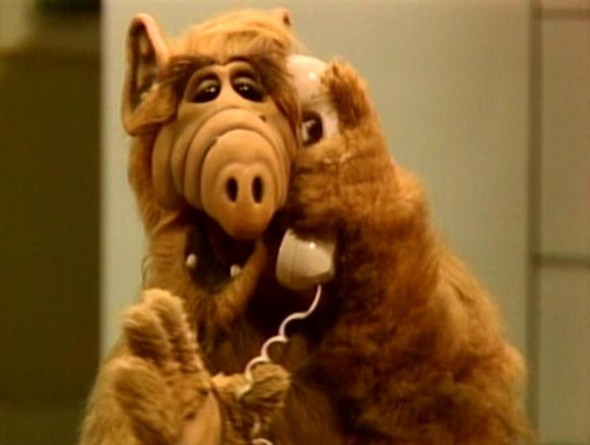
\includegraphics[width=0.9\linewidth]{images/alf.jpg}};
      %   }
      %   \end{column}
      %   \begin{column}{0.32\linewidth}
      %     \footnotesize
      %         Kai Brügge, \\
      %         Astroparticle Physics, \\
      %         TU Dortmund \\
      %         \texttt{kai.bruegge@udo.edu}
      %   \end{column}
      %   \begin{column}{0.18\linewidth}
      %     \tikz[]{
      %       \node[anchor=north]{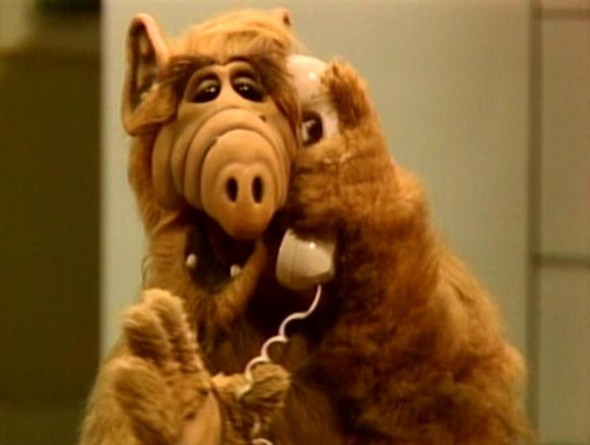
\includegraphics[width=0.9\linewidth]{images/alf.jpg}};
      %   }
      %   \end{column}
      %   \begin{column}{0.32\linewidth}
      %     \footnotesize
      %         Alexey Egorov, \\
      %         Artifical Intelligence Group, \\
      %         TU Dortmund \\
      %         \texttt{alexey.egorov@udo.edu}
      %   \end{column}
      % \end{columns}
    \end{block}

  \end{column}%
\end{columns}%
\end{document}
